\section{Môi trường và cấu trúc mã nguồn}
Ứng dụng dùng Community CLI, không dùng Expo. Các thành phần gồm React Native 0.86.2, React 19.2.3, Async Storage 3.1.1, TypeScript 5.9.3 và Jest 29. package.json yêu cầu Node từ 22.11.0. Android cấu hình SDK 36, Kotlin 2.1.20 và native module riêng; backend dùng Java 17/Maven/Spring Boot 3.4.4.

\subsection{Cấu hình công cụ và điều kiện tái lập}
Bảng~\ref{tab:build-config} trình bày công cụ và cấu hình để cài đặt, build và tái lập ứng dụng. Hệ điều hành của thiết bị chạy thử được nêu tại mục 5.1.
{\tabletext\renewcommand{\arraystretch}{1.04}\begin{longtable}{>{\raggedright\arraybackslash}p{\dimexpr0.19\textwidth-2\tabcolsep\relax}>{\raggedright\arraybackslash}p{\dimexpr0.29\textwidth-2\tabcolsep\relax}>{\raggedright\arraybackslash}p{\dimexpr0.52\textwidth-2\tabcolsep\relax}}
\caption{Công cụ và cấu hình biên dịch}\label{tab:build-config}\\
\toprule \textbf{Hạng mục} & \textbf{Cấu hình biên dịch} & \textbf{Tệp đối chiếu}\\\midrule
\endfirsthead
\multicolumn{3}{l}{\small Công cụ và cấu hình biên dịch (tiếp)}\\
\toprule \textbf{Hạng mục} & \textbf{Cấu hình biên dịch} & \textbf{Tệp đối chiếu}\\\midrule
\endhead
\bottomrule\endlastfoot
Node/npm & Node từ 22.11.0; npm cài theo lockfile & \code{code/booking_classroom/package.json}; \code{package-lock.json}.\\\addlinespace[1.5pt]
Android & Compile/target SDK 36; min SDK 24; Build-Tools 36.0.0 & \code{android/build.gradle}; \code{android/app/build.gradle}, tính từ thư mục app.\\\addlinespace[1.5pt]
Native build & NDK 27.1.12297006; Kotlin 2.1.20; Gradle wrapper 9.3.1 & \code{android/build.gradle}; \code{android/gradle/wrapper/gradle-wrapper.properties}.\\\addlinespace[1.5pt]
Bản Android & Package com.bookingclassroom; versionName 1.0; versionCode 1 & \code{android/app/build.gradle}; version npm 0.0.1 là trường riêng trong package.json.\\\addlinespace[1.5pt]
Backend & Java 17; Spring Boot 3.4.4; H2 file mặc định & \code{code/booking-server/pom.xml}; \code{src/main/resources/application.properties}.\\\addlinespace[1.5pt]
\end{longtable}}

Máy build cần JDK, Android SDK và Platform-Tools/ADB được cấu hình đúng đường dẫn; Windows dùng PowerShell cho script hiện có. Các phiên bản và tên thiết bị trong hồ sơ kiểm thử được trình bày riêng ở Chương~\ref{chap:testing}.

\subsection{Cấu trúc mã nguồn và trách nhiệm triển khai}

Các đường dẫn trong chương tính từ repository \code{final_project/}. Mã nguồn ứng dụng ở \code{code/booking_classroom/}, backend ở \code{code/booking-server/}. Cấu trúc thực tế được tóm tắt như sau:
{\small\renewcommand{\arraystretch}{1.1}
\begin{longtable}{>{\raggedright\arraybackslash}p{\dimexpr.49\textwidth-2\tabcolsep\relax}>{\raggedright\arraybackslash}p{\dimexpr.51\textwidth-2\tabcolsep\relax}}
\caption{Cấu trúc thư mục và trách nhiệm}\label{tab:source-tree}\\
\toprule\textbf{Vị trí trong repository} & \textbf{Vai trò}\\\midrule
\endfirsthead
\multicolumn{2}{l}{Cấu trúc thư mục và trách nhiệm (tiếp)}\\
\toprule\textbf{Vị trí trong repository} & \textbf{Vai trò}\\\midrule
\endhead
\bottomrule\endlastfoot
\code{code/booking_classroom/App.tsx} & Điểm ghép giao diện và phiên của app.\\\addlinespace[1.5pt]
\code{code/booking_classroom/src/app/} & Ghép màn hình theo vai trò.\\\addlinespace[1.5pt]
\code{code/booking_classroom/src/core/} & API, storage, time, config và types dùng chung.\\\addlinespace[1.5pt]
\code{code/booking_classroom/src/modules/} & 11 module nghiệp vụ.\\\addlinespace[1.5pt]
\code{code/booking_classroom/src/shared/} & Thành phần UI dùng chung.\\\addlinespace[1.5pt]
\code{code/booking_classroom/android/app/src/} & Native Android.\\\addlinespace[1.5pt]
\code{code/booking_classroom/__tests__/}; \code{code/booking_classroom/quality-tests/} & Test ứng dụng và bộ kiểm thử chất lượng riêng.\\\addlinespace[1.5pt]
\code{code/booking-server/src/main/java/} & Gói com/bookingclassroom/server/: service, entity, session; thư mục api/ có sáu controller.\\\addlinespace[1.5pt]
\code{code/booking-server/src/main/resources/} & Cấu hình backend.\\\addlinespace[1.5pt]
\code{code/booking-server/src/test/} & Kiểm thử tích hợp H2.\\
\end{longtable}}

Màn hình tiếp nhận thao tác và hiển thị dữ liệu; dịch vụ kiểm tra nghiệp vụ trước khi đọc/ghi qua repository. Model xác định kiểu dữ liệu trao đổi. Nghiệp vụ đặt phòng phối hợp với phòng, cấu hình, bảo trì, cấp quyền, tự duyệt và thông báo; phép kiểm giao thời gian được dùng chung để giữ nhất quán.

\section{Ánh xạ yêu cầu chức năng tới mã nguồn}
Trong Bảng~\ref{tab:fr-code}, tiền tố file app là \code{code/booking_classroom/}; phần tên hàm mô tả điểm triển khai cụ thể.
{\tabletext\renewcommand{\arraystretch}{1.04}\begin{longtable}{>{\raggedright\arraybackslash}p{\dimexpr0.08\textwidth-2\tabcolsep\relax}>{\raggedright\arraybackslash}p{\dimexpr0.49\textwidth-2\tabcolsep\relax}>{\raggedright\arraybackslash}p{\dimexpr0.43\textwidth-2\tabcolsep\relax}}
\caption{Ánh xạ chức năng, vị trí và bằng chứng}\label{tab:fr-code}\\
\toprule \textbf{FR} & \textbf{Màn hình / vị trí xử lý} & \textbf{Hành vi và minh chứng}\\\midrule
\endfirsthead
\multicolumn{3}{l}{\small Ánh xạ chức năng, vị trí và bằng chứng (tiếp)}\\
\toprule \textbf{FR} & \textbf{Màn hình / vị trí xử lý} & \textbf{Hành vi và minh chứng}\\\midrule
\endhead
\bottomrule\endlastfoot
FR01 & \code{src/modules/auth/screens/LoginScreen.tsx}; \code{src/modules/auth/services/accountRepository.ts}. & Đăng nhập cập nhật phiên và mở màn hình đúng vai trò; đăng ký, đổi/khôi phục mật khẩu kiểm dữ liệu và phản hồi lỗi. TC01, TC17; D01--D03.\\\addlinespace[1.5pt]
FR02 & \code{src/modules/room_management/screens/RoomSearchScreen.tsx}; \code{src/modules/room_management/services/roomRepository.ts}. & Bộ lọc kết hợp danh mục, booking và bảo trì để hiển thị phòng khả dụng. Hình~\ref{fig:ui-booking}; TC02, TC12.\\\addlinespace[1.5pt]
FR03 & \code{src/modules/booking/services/bookingRepository.ts}; \code{src/modules/booking/screens/MyBookingsScreen.tsx}. & Kiểm từng lượt trước khi lưu chuỗi; hủy/sửa theo quyền, trạng thái và hạn chót. TC11--TC12, TC21.\\\addlinespace[1.5pt]
FR04 & \code{src/modules/booking/screens/AdminBookingScreen.tsx}; \code{src/modules/auto_approval/model/approvalPolicy.ts}. & Duyệt tay theo quyền admin; tự duyệt sau kiểm tra hợp lệ khi phòng thường và cấu hình cho phép. TC07, TC20, TC24.\\\addlinespace[1.5pt]
FR05 & \code{src/modules/access_control/services/temporaryPinService.ts}; \code{src/modules/booking/services/bookingRepository.ts}. & Kiểm chủ lượt/quyền phòng, lưu PIN và gửi qua OneIoT; trao đổi lịch nhận chìa và ủy quyền. TC03, TC10, TC13--TC15, TC19.\\\addlinespace[1.5pt]
FR06 & \code{src/modules/smart_lock/services/smartLockAccessEventService.ts}; \code{src/modules/booking/services/bookingRepository.ts}. & Tiếp nhận sự kiện khóa, ghi nhận có mặt/ra và chặn no-show khi đã có check-in. TC10, TC22.\\\addlinespace[1.5pt]
FR07 & \code{src/modules/schedule_maintenance/services/maintenanceRepository.ts}; \code{src/modules/booking/services/bookingRepository.ts}. & Tách ghi chú, yêu cầu bảo trì và lịch chặn phòng; admin xử lý theo trạng thái. TC02, TC23.\\\addlinespace[1.5pt]
FR08 & \code{src/modules/account_management/}; \code{src/modules/configuration/}; \code{src/modules/profile/}; \code{src/modules/notifications/}. & Quản trị theo quyền; lưu hồ sơ/cấu hình và thông báo theo người nhận. TC06, TC08--TC09, TC16, TC18.\\\addlinespace[1.5pt]
\end{longtable}}

Màn tìm và đặt nằm trong room\_management nhưng gọi nghiệp vụ booking; quản lý tài khoản có UI riêng nhưng dùng accountRepository của auth. Phân quyền online được kiểm thêm ở filter/service Java, không dựa riêng vào việc UI ẩn nút.

\Needspace{13\baselineskip}
\section{Ma trận kỹ thuật React Native}
{\tabletext\renewcommand{\arraystretch}{1.04}\begin{longtable}{>{\raggedright\arraybackslash}p{\dimexpr0.19\textwidth-2\tabcolsep\relax}>{\raggedright\arraybackslash}p{\dimexpr0.55\textwidth-2\tabcolsep\relax}>{\raggedright\arraybackslash}p{\dimexpr0.26\textwidth-2\tabcolsep\relax}}
\caption{Kỹ thuật, cách áp dụng, lý do và kiểm chứng}\label{tab:rn}\\
\toprule \textbf{Kỹ thuật} & \textbf{Vị trí và cách áp dụng / lý do} & \textbf{Bằng chứng}\\\midrule
\endfirsthead
\multicolumn{3}{l}{\small Kỹ thuật, cách áp dụng, lý do và kiểm chứng (tiếp)}\\
\toprule \textbf{Kỹ thuật} & \textbf{Vị trí và cách áp dụng / lý do} & \textbf{Bằng chứng}\\\midrule
\endhead
\bottomrule\endlastfoot
Component, JSX, Props & \code{App.tsx}: App truyền session/onLogout cho RoleDashboardScreen và onLogin cho LoginScreen. Props/callback tập trung phiên ở gốc, tránh sao chép trạng thái xác thực. & Đoạn A; TC01, D02.\\\addlinespace[1.5pt]
State & \code{src/modules/auth/screens/LoginScreen.tsx}: LoginScreen dùng useState cho input, error và submitting. Trạng thái cục bộ đáp ứng biểu mẫu; useReducer không áp dụng. & TC01, TC17; D01--D03.\\\addlinespace[1.5pt]
Effect và cleanup & \code{App.tsx}: App.useEffect đăng ký AppState/sự kiện khóa rồi tháo listener và ngắt MQTT; \code{src/modules/auth/screens/LoginScreen.tsx}: effect xử lý BackHandler. Cleanup tránh lặp bộ lắng nghe khi chuyển màn. & App, dòng 24--38; kiểm thử bridge và callback.\\\addlinespace[1.5pt]
Custom Hook / Context / Store & Không áp dụng ở tầng nghiệp vụ: quy mô hiện tại dùng state cục bộ, props và service; chưa cần store dùng chung. & Cấu trúc phụ thuộc ở mục 4.1; đoạn A.\\\addlinespace[1.5pt]
Điều hướng & \code{src/app/screens/RoleDashboardScreen.tsx}: RoleDashboardScreen dùng activeScreen, closeChildScreen và onBack; giữ điều hướng tập trung cho số màn hiện tại. & Hình~\ref{fig:flow-user}--\ref{fig:flow-admin}; D02.\\\addlinespace[1.5pt]
Async, API, Promise & \code{src/core/api/client.ts}: apiRequest dùng fetch, AbortController và finally; tập trung token, giới hạn chờ và chuyển lỗi cho UI. & Đoạn B; TC04--TC05.\\\addlinespace[1.5pt]
Form và validation & \code{src/modules/auth/screens/LoginScreen.tsx}: submit kiểm dữ liệu, đặt submitting, gọi authenticate và khôi phục trạng thái trong finally; kiểm lại ở service để bảo vệ nghiệp vụ. & TC01, TC17; D01, D03.\\\addlinespace[1.5pt]
Danh sách & \code{src/modules/room_management/}\par\code{screens/RoomSearchScreen.tsx}: RoomSearchScreen dùng ScrollView/map và key theo định danh, phù hợp danh mục hiện tại. FlatList/phân trang không áp dụng. & Hình~\ref{fig:ui-booking}; kiểm thử bộ lọc.\\\addlinespace[1.5pt]
Lưu trữ và quyền & \code{src/core/storage/jsonStorage.ts}: readJson/writeJson bọc Async Storage; \code{src/modules/notifications/services/priorityBanner.ts}: requestPriorityNotificationPermission xử lý API 33+. Tách lưu trữ khỏi UI và xin quyền theo nền tảng. & TC08--TC09; D05--D06.\\\addlinespace[1.5pt]
Tối ưu / nền tảng & \code{src/app/screens/RoleDashboardScreen.tsx}: refreshUnreadCount dùng useCallback để ổn định dependency của effect; \code{src/modules/notifications/services/priorityBanner.ts} kiểm Platform.OS trước khi gọi native. & Kiểm thử quyền API 31/33 và bản chạy Android.\\\addlinespace[1.5pt]
\end{longtable}}

\section{Phân tích hai đoạn mã cốt lõi}
\par\noindent\begin{minipage}{\linewidth}
\setlength{\parindent}{1cm}
\subsection{Đoạn A: giao diện, phiên và callback}
\textbf{Tệp:} \coderef{code/booking_classroom/App.tsx}, dòng 40--62. Liên quan FR01/FR08 và G03. Đầu vào là session do useState ở dòng 18 giữ; đầu ra là cây component theo trạng thái xác thực.
\VerbatimInput[fontsize=\small,numbers=left,numbersep=5pt,firstnumber=40,firstline=40,lastline=62,breaklines=true,frame=single]{../../../../code/booking_classroom/App.tsx}

\end{minipage}\par\smallskip
\textbf{Phân tích.} Dòng 47 rẽ nhánh bằng session; 48--55 truyền dữ liệu và callback cho màn theo vai trò. Dòng 50--53 gom logout: ngắt OneIoT, xóa token, đặt session null. Dòng 57 truyền setSession làm onLogin; khi LoginScreen hoàn tất authenticate, callback làm App render lại. Props/callback duy trì một chủ sở hữu phiên, không sao chép mật khẩu vào state toàn app.

Trạng thái lỗi/loading thuộc LoginScreen: submit kiểm ô trống, đặt submitting, xử lý null/error rồi khôi phục trạng thái trong finally. Effect tại App dòng 24--38 đăng ký listener và dọn dẹp khi unmount/xuống nền \cite{react}. Người dùng đăng nhập lại sau khi mở ứng dụng; MQTT hoạt động theo phiên kết nối. App.test/authScreens kiểm giao diện và điều hướng; thử nghiệm trên thiết bị xác nhận quá trình sử dụng cùng SmartLock.

\par\noindent\begin{minipage}{\linewidth}
\setlength{\parindent}{1cm}
\subsection{Đoạn B: xử lý HTTP bất đồng bộ và ngoại lệ}
\textbf{Tệp:} \coderef{code/booking_classroom/src/core/api/client.ts}, dòng 35--61. Liên quan FR01--FR08/NFR02. Đầu vào là path, method, body và token của phiên; đầu ra là response JSON hoặc Error cho màn hình.
\VerbatimInput[fontsize=\small,numbers=left,numbersep=5pt,firstnumber=35,firstline=35,lastline=61,breaklines=true,frame=single]{../../../../code/booking_classroom/src/core/api/client.ts}

\end{minipage}\par\smallskip
\textbf{Phân tích.} Dòng 36--37 tạo controller và timer giới hạn chờ. Dòng 39--42 chuẩn hóa/kiểm URL; 43--52 đóng gói request, thêm Bearer nếu có, serialize body và gắn signal. Dòng 53--58 chuyển lỗi mạng/abort thành thông điệp nghiệp vụ; finally 59--61 xóa timer dù thành công hay lỗi.

Phần sau trích đoạn xử lý 204, parse JSON, thông báo lỗi HTTP và xóa token khi 401. Client không tự retry để tránh lặp thao tác ghi, không tự fallback local vì hai kho không hòa giải. Kiểm thử HTTP mô phỏng fetch và timer để xác nhận header, body, lỗi JSON, lỗi 401, mất mạng và ngắt yêu cầu sau 12 giây (TC04--TC05). Đây là kiểm tra cơ chế giới hạn chờ ở client.

\Needspace{17\baselineskip}
\section{Truy vết luồng đăng nhập và xử lý ngoại lệ}
{\tabletext\renewcommand{\arraystretch}{1.04}\begin{longtable}{>{\raggedright\arraybackslash}p{\dimexpr0.3\textwidth-2\tabcolsep\relax}>{\raggedright\arraybackslash}p{\dimexpr0.44\textwidth-2\tabcolsep\relax}>{\raggedright\arraybackslash}p{\dimexpr0.26\textwidth-2\tabcolsep\relax}}
\caption{Từ thao tác tới render trong luồng đăng nhập}\label{tab:trace}\\
\toprule \textbf{Bước / vị trí} & \textbf{Dữ liệu và trạng thái} & \textbf{Kiểm chứng}\\\midrule
\endfirsthead
\multicolumn{3}{l}{\small Từ thao tác tới render trong luồng đăng nhập (tiếp)}\\
\toprule \textbf{Bước / vị trí} & \textbf{Dữ liệu và trạng thái} & \textbf{Kiểm chứng}\\\midrule
\endhead
\bottomrule\endlastfoot
1. LoginScreen onChange/submit & TextInput cập nhật username/password. Thiếu ô bắt buộc đặt error; không gửi request. & AuthScreens quality và giao diện đăng nhập.\\\addlinespace[1.5pt]
2. submit / authenticate & submitting=true, xóa/ghi error theo kết quả; local đọc auth.accounts hoặc REST gọi login. & Auth unit/component; apiClient mock.\\\addlinespace[1.5pt]
3. accountRepository / apiRequest & REST nhận token/role; lỗi xác thực trả null theo điều kiện. Mạng lỗi/timeout thành Error, 401 xóa token. & Test sai mật khẩu, duplicate và các ca API lỗi.\\\addlinespace[1.5pt]
4. onLogin / App.setSession & Thành công truyền username/role, render RoleDashboard theo role; không truyền mật khẩu. & App.test; biên bản Admin/User.\\\addlinespace[1.5pt]
5. finally / cleanup & submitting=false để mở lại nút. BackHandler/listener bị tháo khi màn tương ứng đóng; logout/ngắt nền đóng MQTT. & Source submit/useEffect; native bridge được mock.\\\addlinespace[1.5pt]
\end{longtable}}

Khi xác thực thất bại hoặc mất kết nối REST, ứng dụng giữ người dùng ở biểu mẫu và hiển thị thông điệp lỗi cụ thể. Dữ liệu local thiếu được repository khởi tạo theo model; dữ liệu remote lỗi định dạng bị API client từ chối. Các màn giữ loading/error bằng state; cập nhật state làm component render lại.

\section{Giao diện và sản phẩm chạy thử}
Chín ảnh giao diện minh họa các bước thao tác và nhóm chức năng của ứng dụng, từ đăng nhập, đặt phòng đến quản lý và cấu hình. Các luồng này được kết hợp kiểm thử tự động và chạy thực tế trên thiết bị.

\subsection{Đăng nhập và phân tách chức năng theo vai trò}
Hình~\ref{fig:ui-roles} gồm đăng nhập và hai dashboard. Kết quả xác thực xác định vai trò và nhóm chức năng hiển thị; tầng dịch vụ tiếp tục kiểm quyền đối với từng thao tác. Đổi tài khoản cập nhật phiên, xóa token REST và ngắt OneIoT khi đăng xuất.

Màn hình đăng nhập sử dụng các trường tài khoản, mật khẩu và thông báo lỗi. Kiểm thử xác thực xác nhận các ô bắt buộc, sai mật khẩu, chuyển biểu mẫu và mở chức năng đúng vai trò (TC01, TC17 và D01--D03).

\begin{figure}[H]\centering
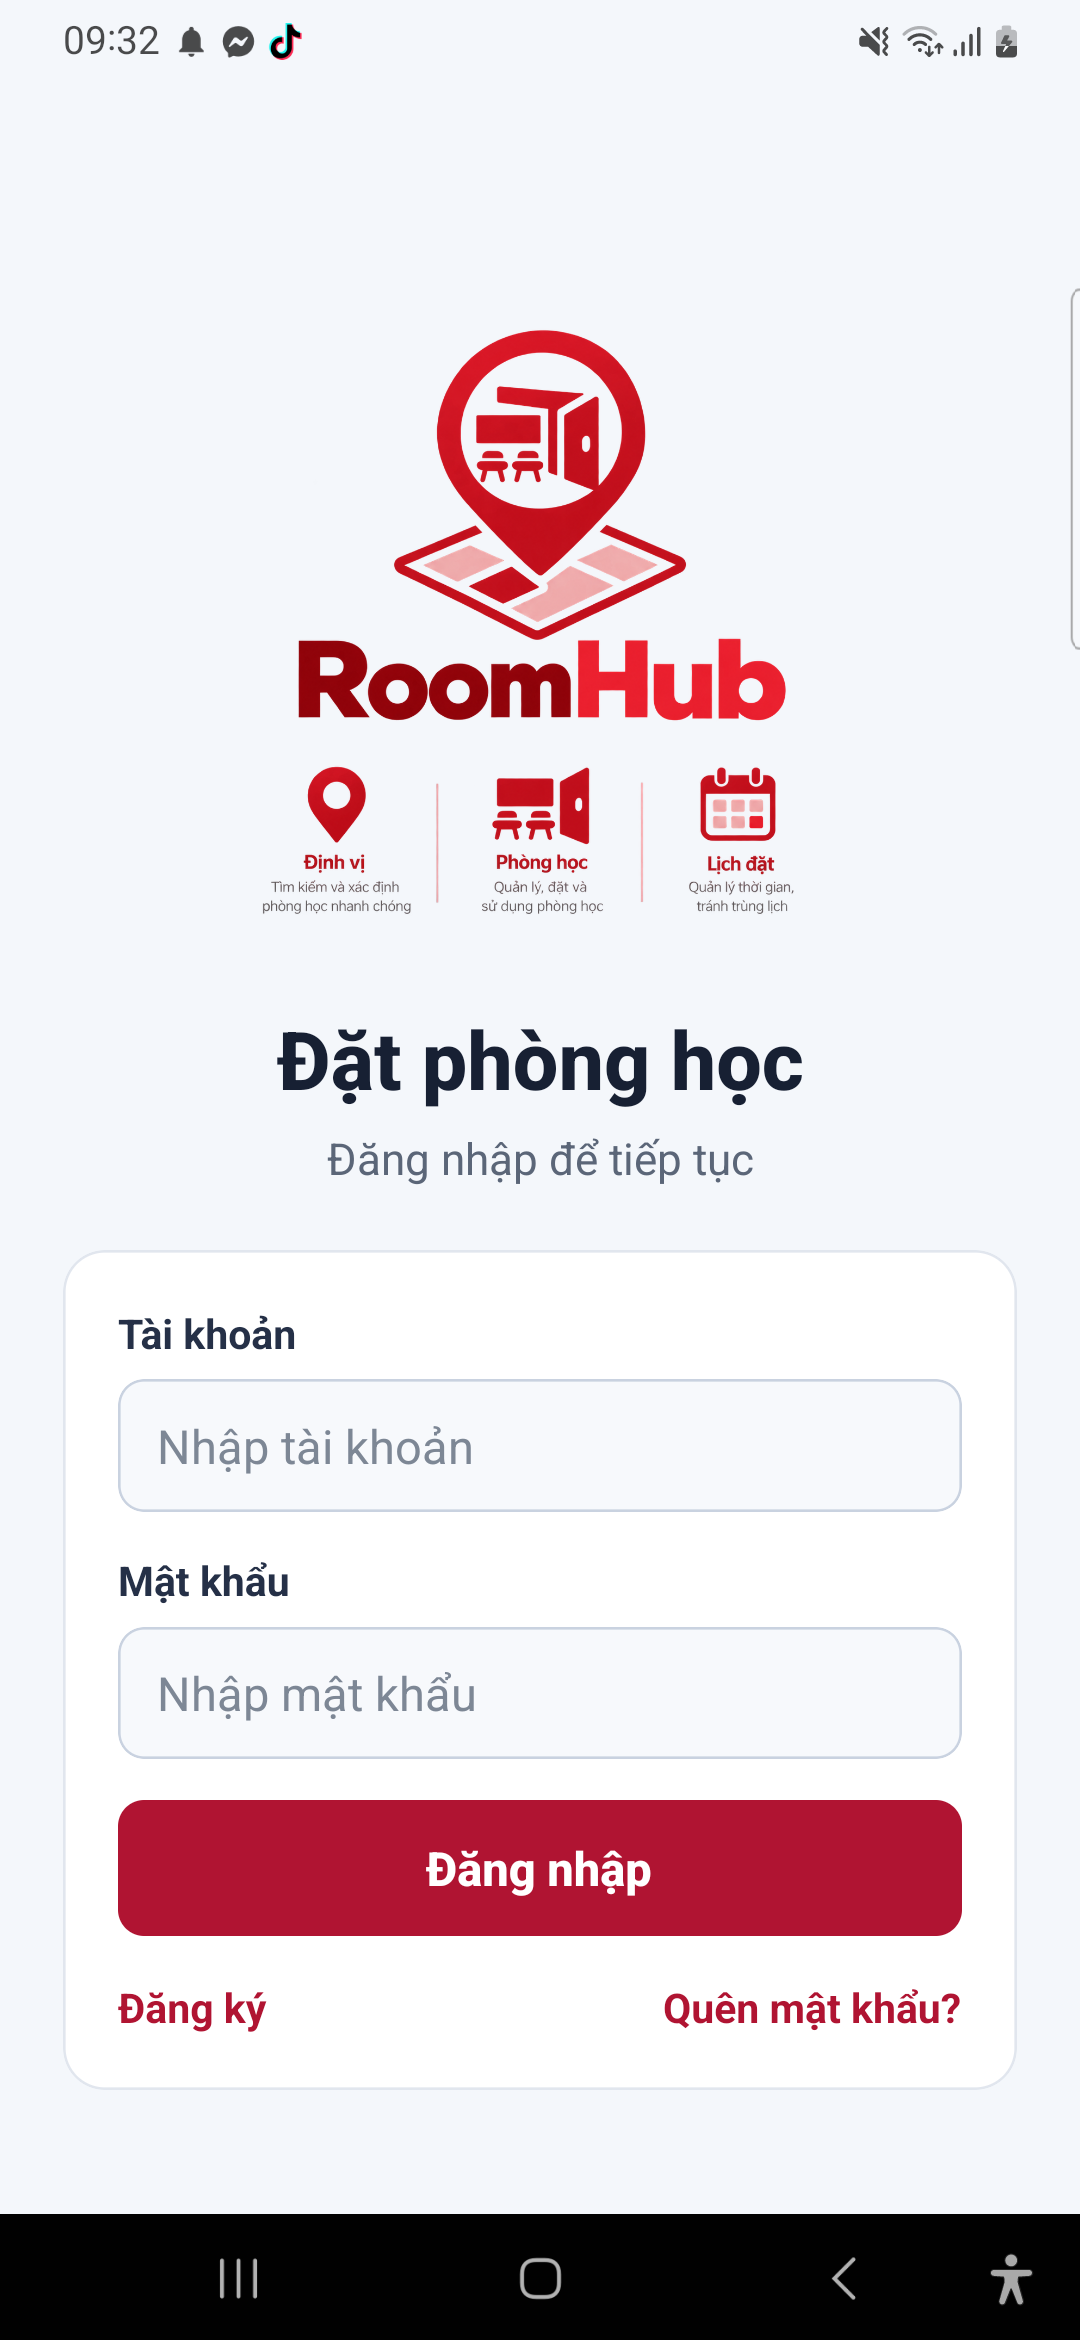
\includegraphics[height=7.8cm]{Hinhve/login_hien_tai.png}\hspace{.6cm}
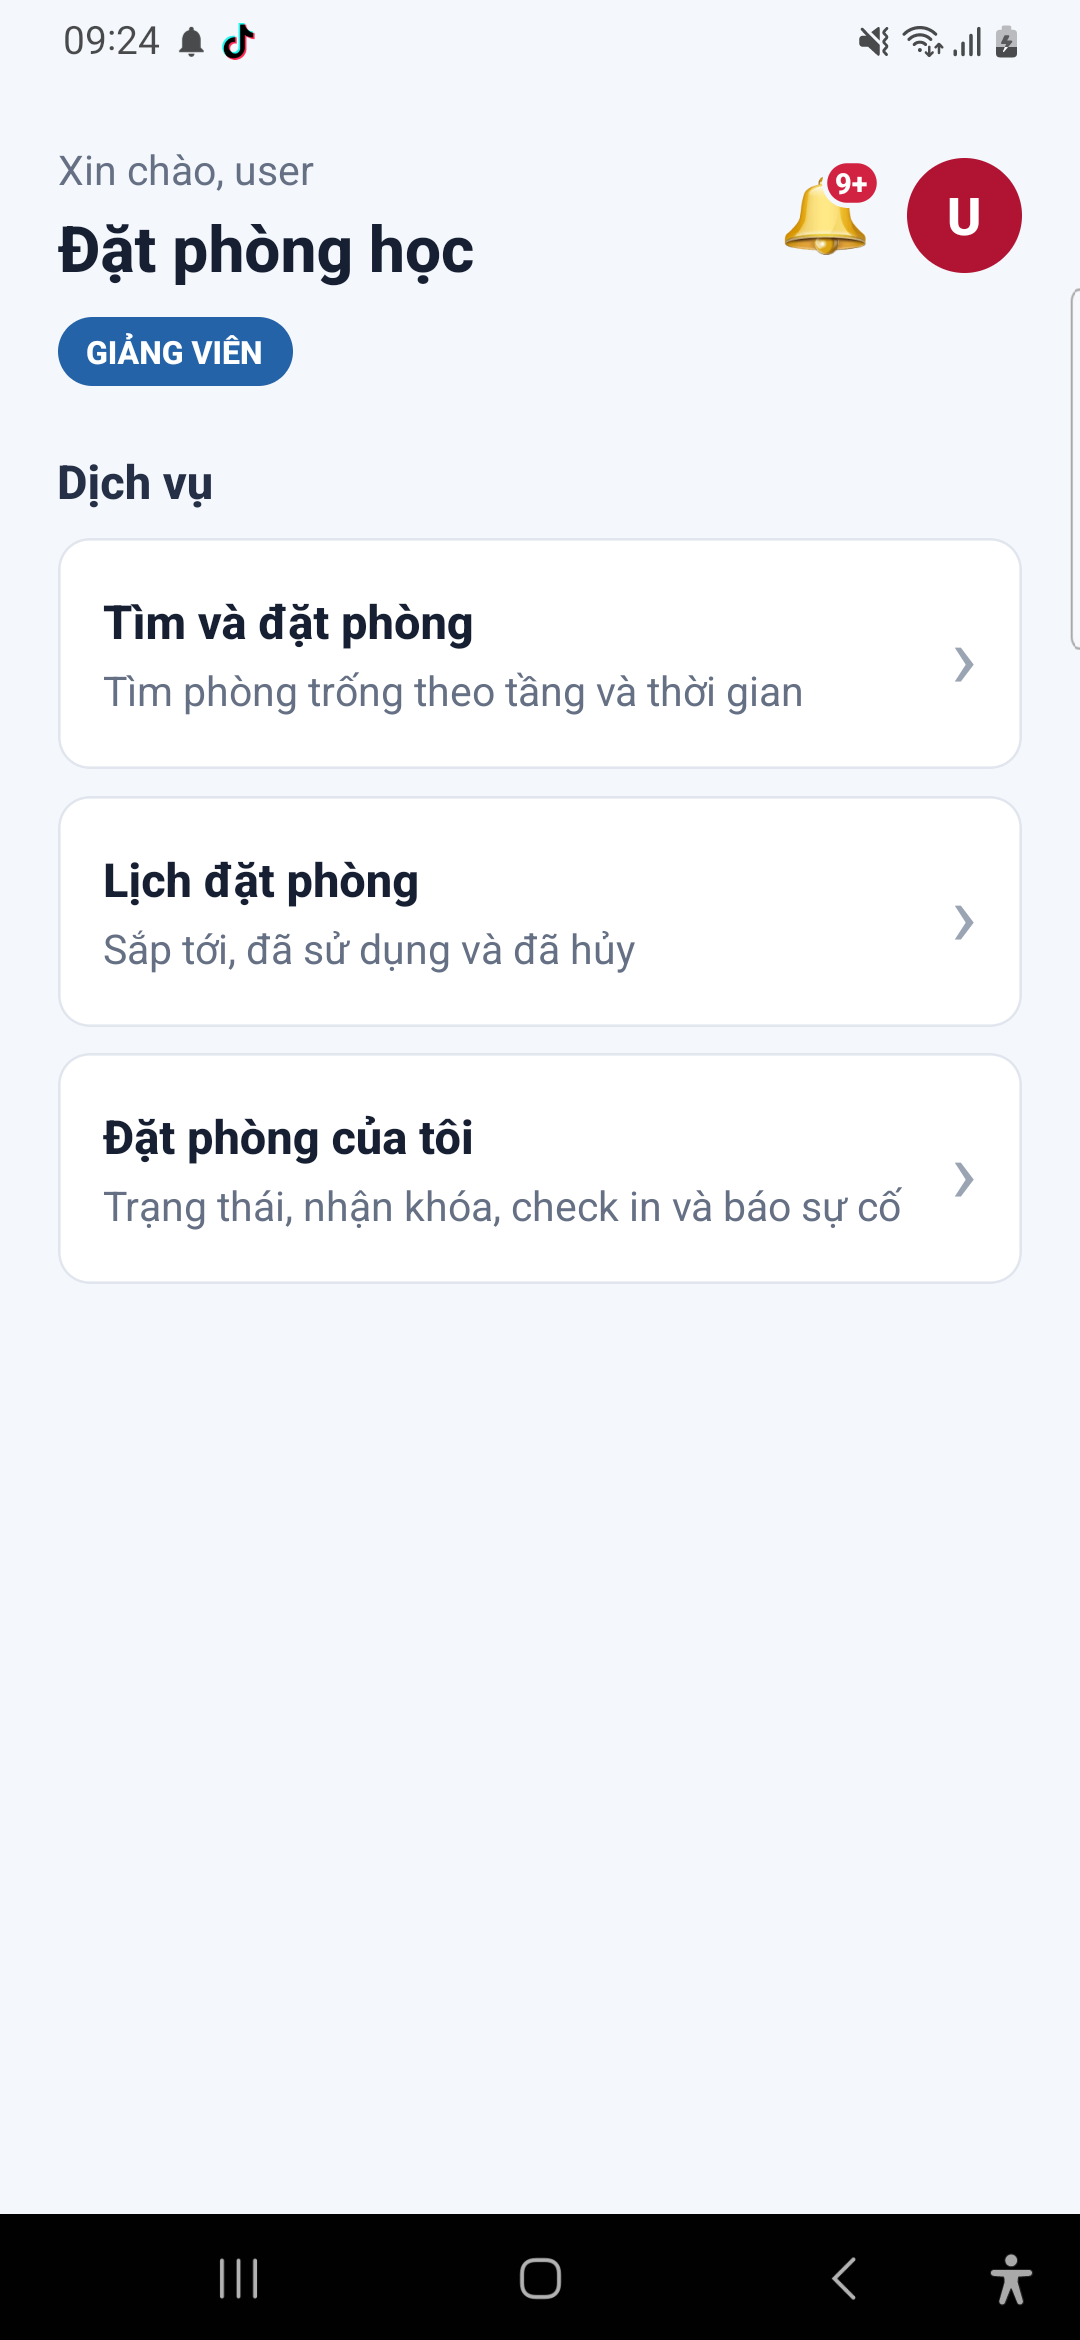
\includegraphics[height=7.8cm]{Hinhve/giao_dien_nguoi_dung_hien_tai.png}\hspace{.6cm}
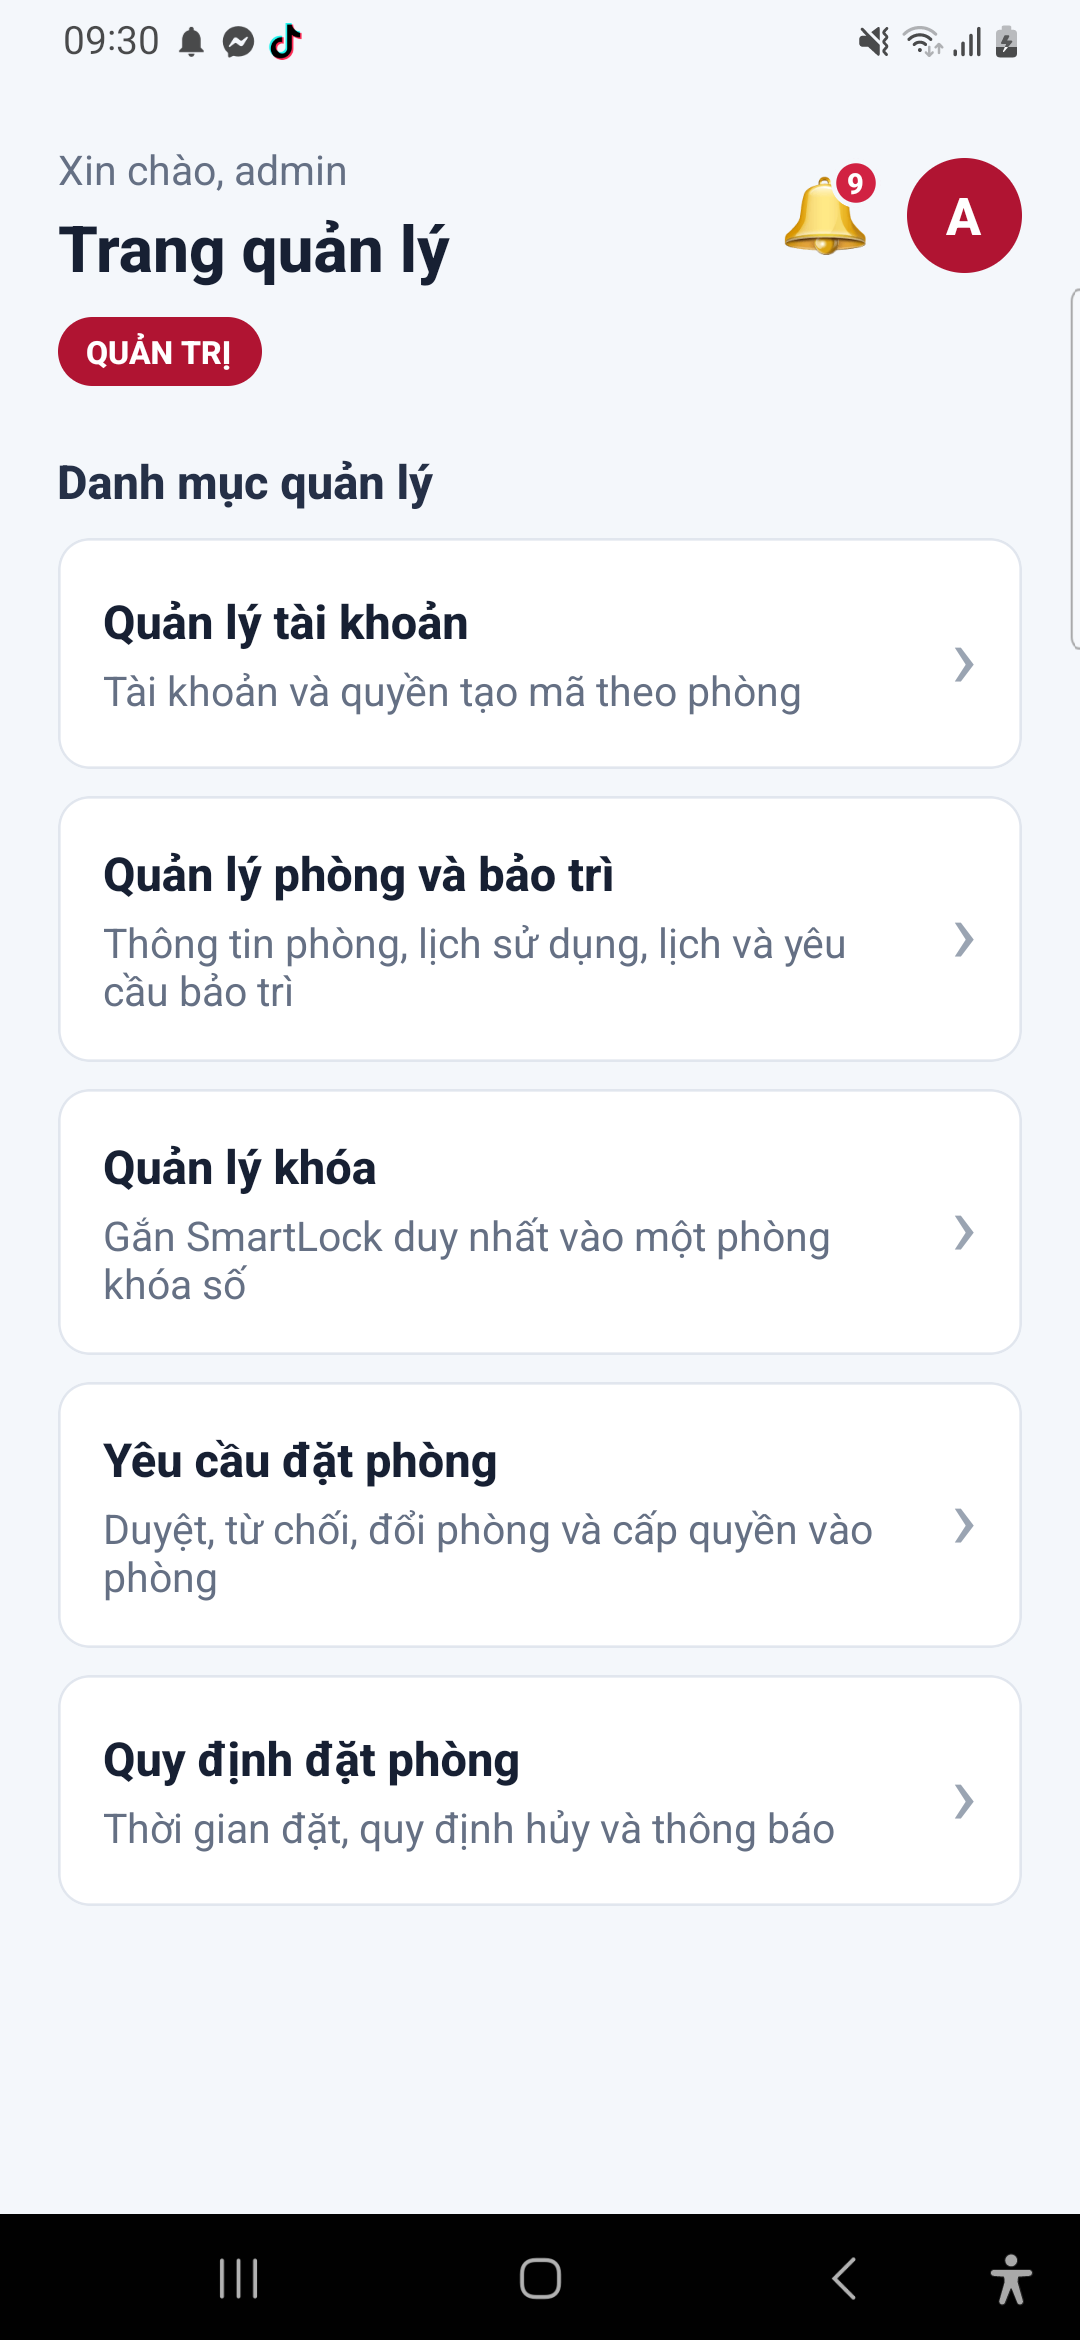
\includegraphics[height=7.8cm]{Hinhve/giao_dien_admin_hien_tai.png}
\caption{Đăng nhập, chức năng User và Admin (trái sang phải)}\label{fig:ui-roles}
\end{figure}
\subsection{Tìm và gửi yêu cầu trên cùng màn hình}
Hình~\ref{fig:ui-booking} giữ hai bước: chọn tầng/ngày/giờ, sức chứa/thiết bị/loại khóa; rồi chọn phòng, nhập mục đích và gửi. Ứng dụng tải danh mục và mức chiếm chỗ để hỗ trợ lựa chọn; khi gửi yêu cầu, tầng nghiệp vụ kiểm lại lịch và các quy tắc trước khi ghi. Tám tầng là dữ liệu demo.

\begin{figure}[H]\centering
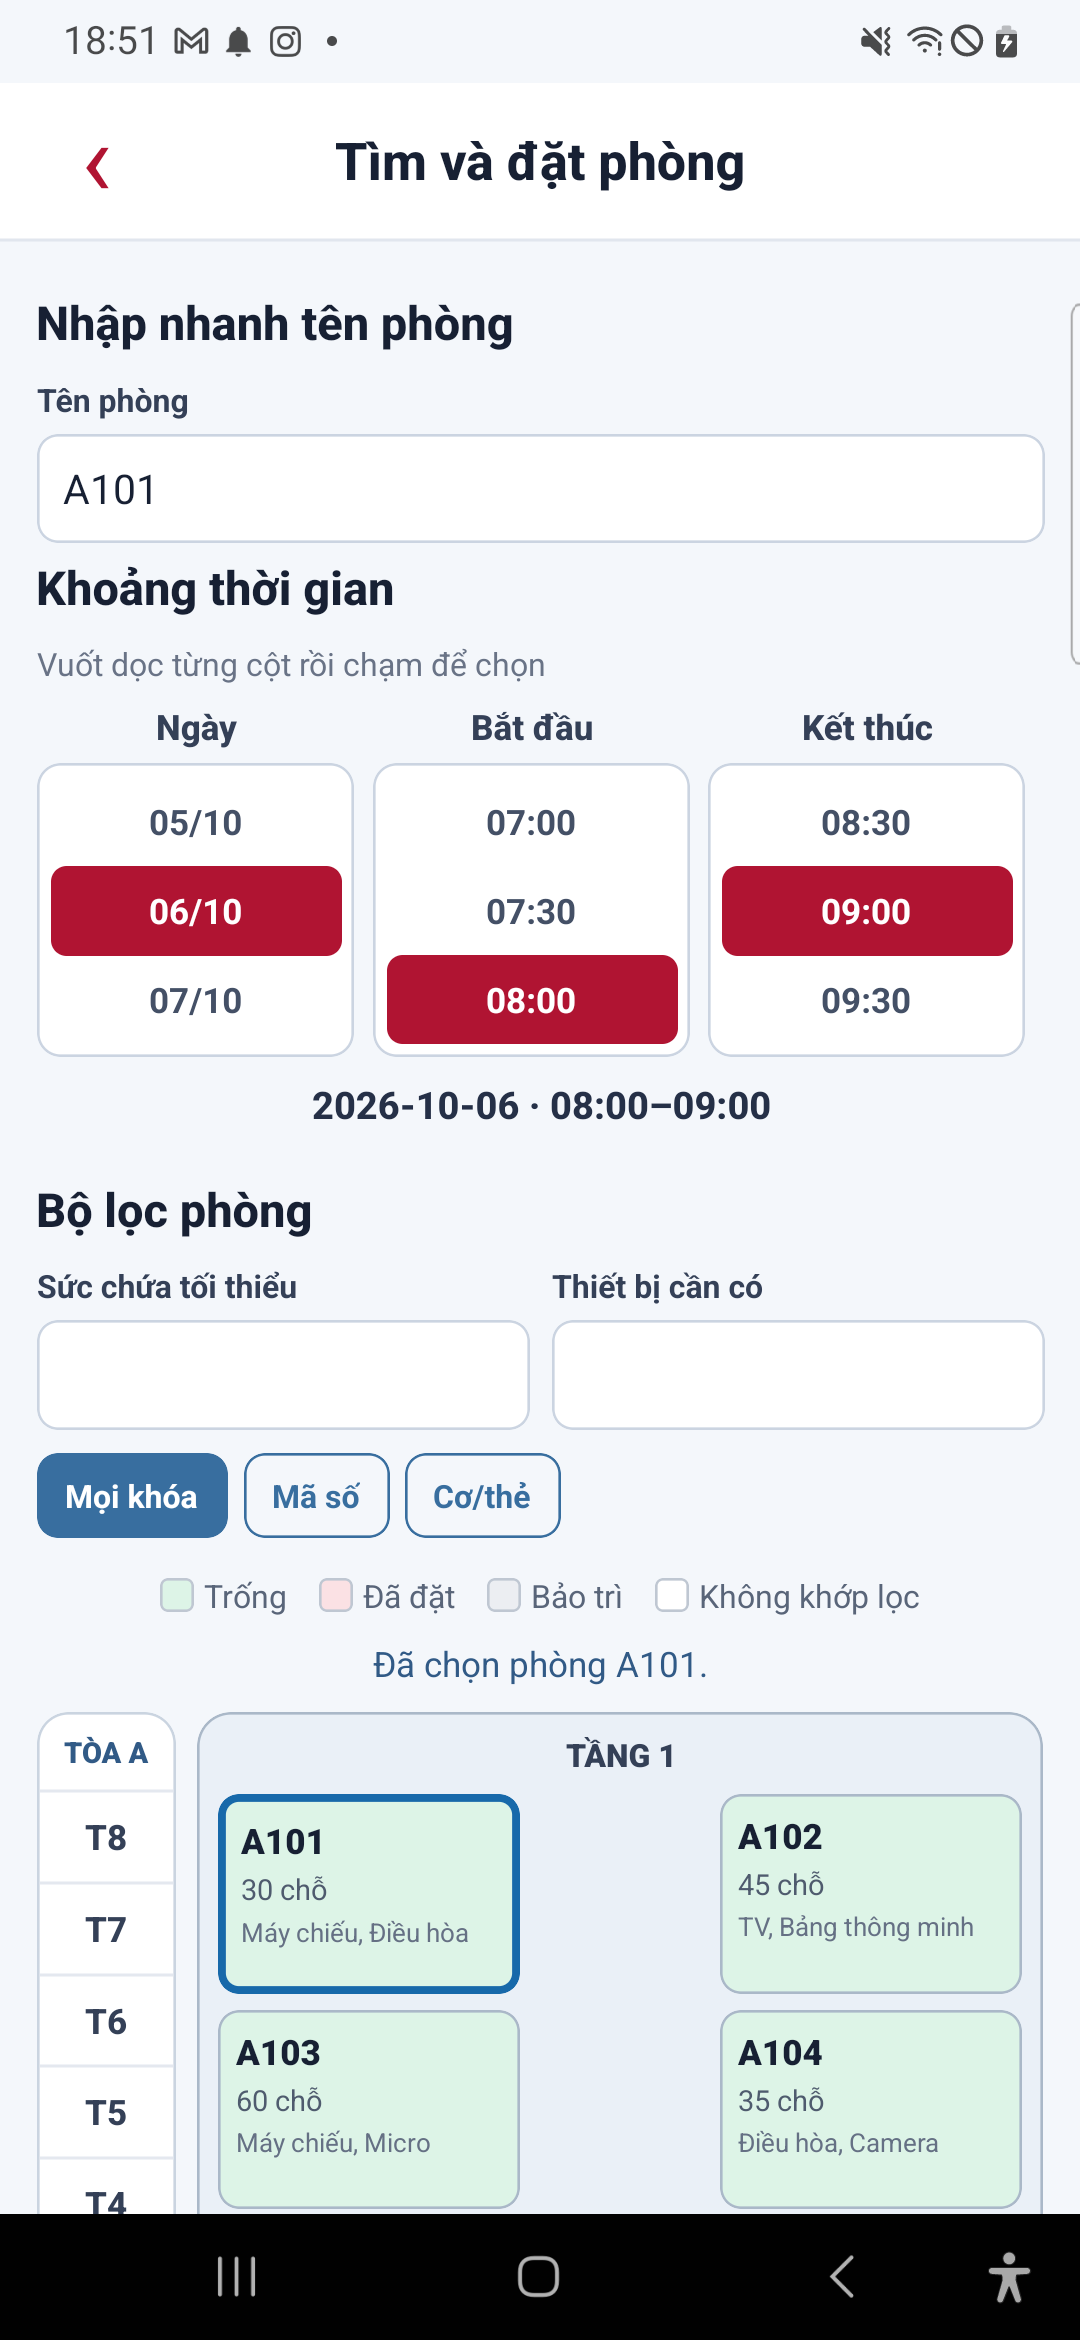
\includegraphics[height=8cm]{Hinhve/tim_va_dat_phong_hien_tai.png}\hspace{1.2cm}
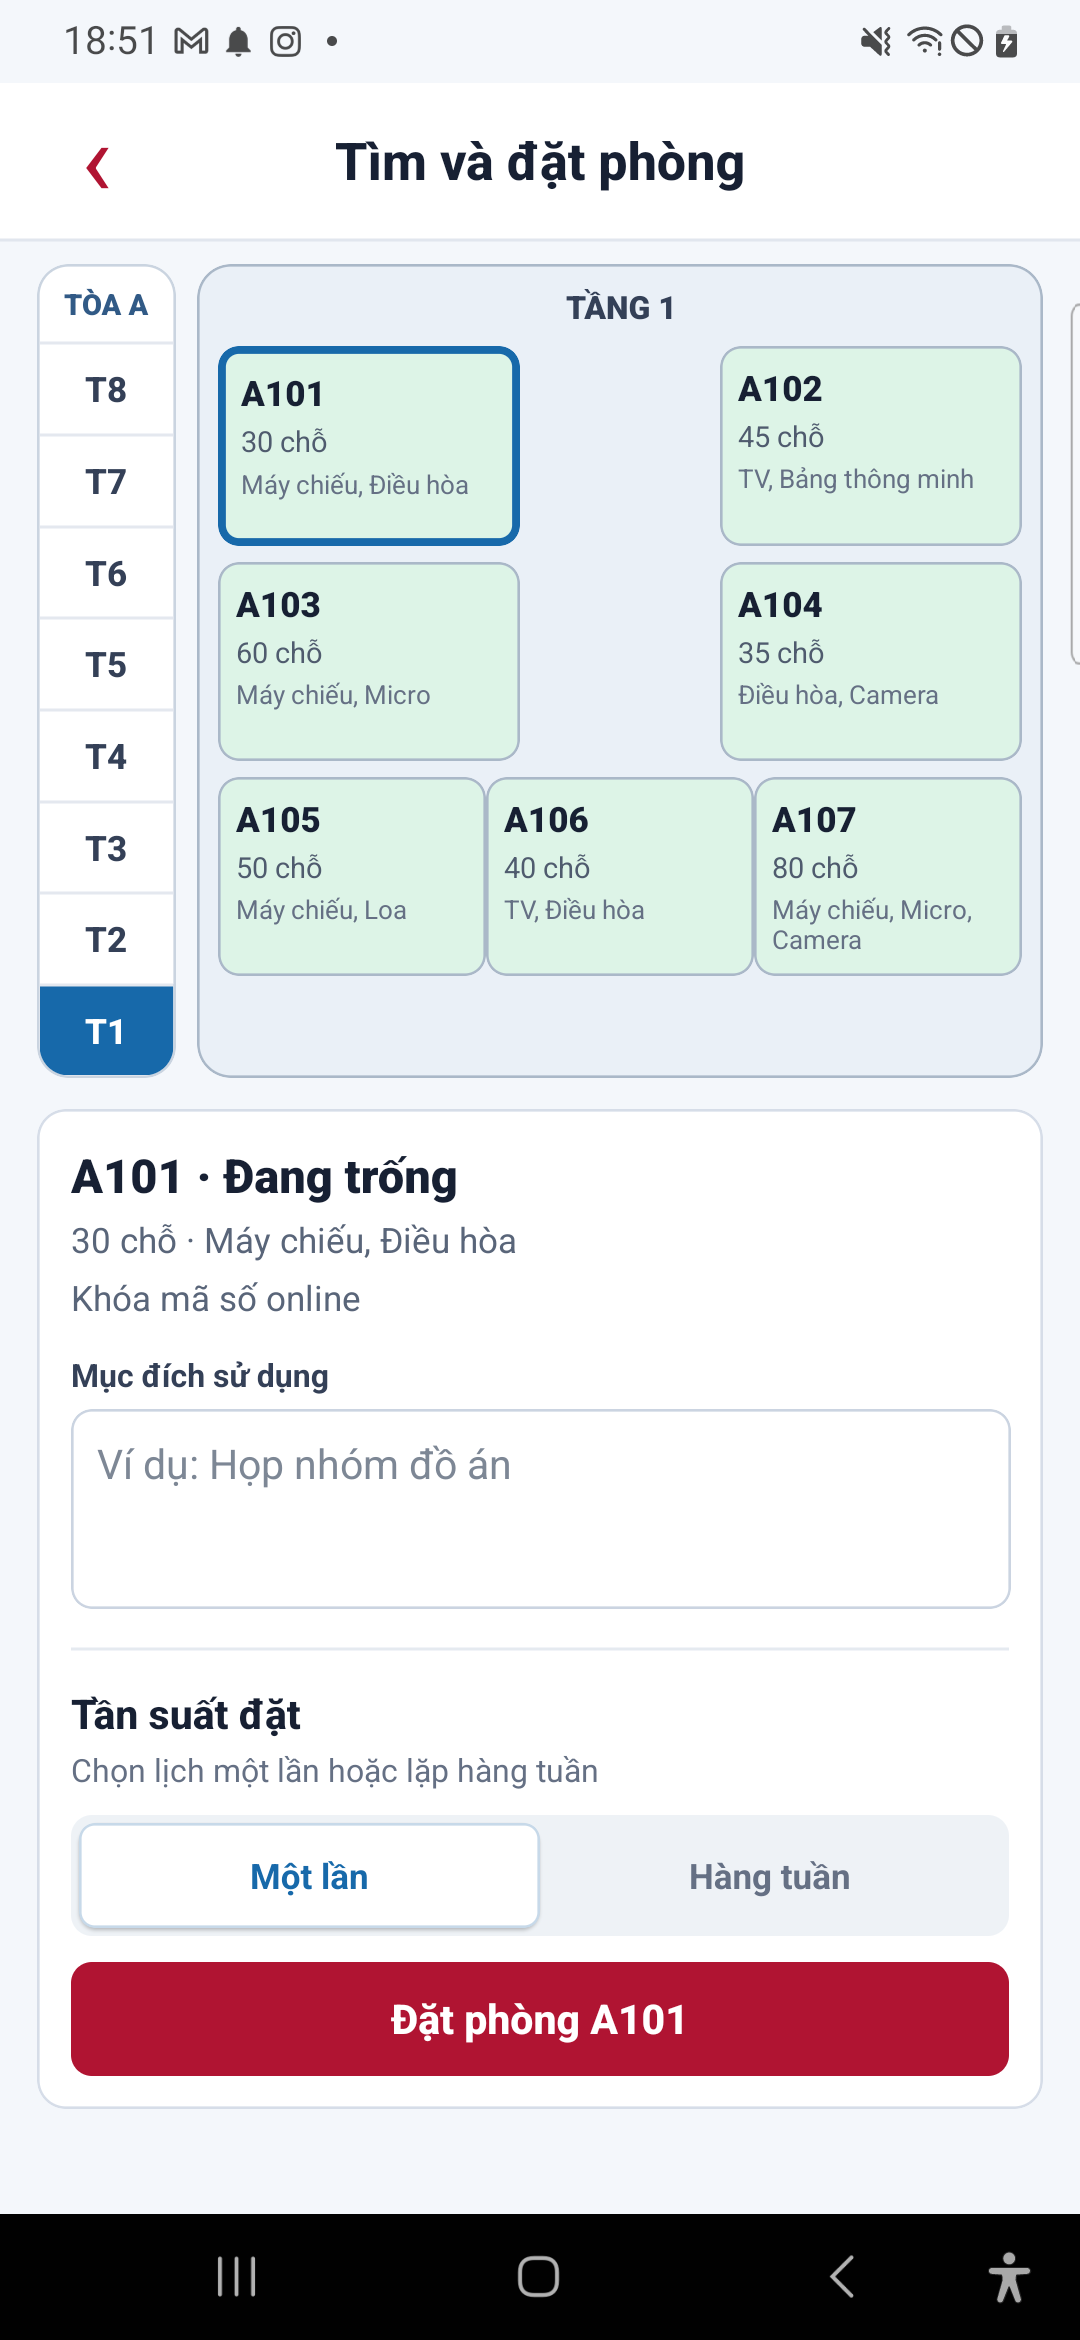
\includegraphics[height=8cm]{Hinhve/chon_phong_va_dat_hien_tai.png}
\caption{Chọn tiêu chí, chọn phòng và gửi yêu cầu (trái sang phải)}\label{fig:ui-booking}
\end{figure}
\subsection{Quản lý phòng và bảo trì theo tầng}
Hình~\ref{fig:ui-room-maintenance} gồm danh sách tầng thu gọn có số phòng/chỉ báo bảo trì và tầng đã mở với thông tin từng phòng. Các tầng có thể mở/thu gọn; trạng thái phòng được tổng hợp từ danh mục, lượt đặt, yêu cầu và lịch bảo trì.

Admin chọn phòng để sửa/xóa, xem hoặc lập/hủy lịch bảo trì. Service chặn xóa phòng còn booking hoạt động; phòng mẫu đã xóa được lưu dấu để không tự tái xuất hiện. Yêu cầu bảo trì phải qua tiếp nhận/lên lịch mới chặn phòng; ghi chú chỉ thông báo admin (UC08, UC13; TC02, TC23).

\begin{figure}[H]\centering
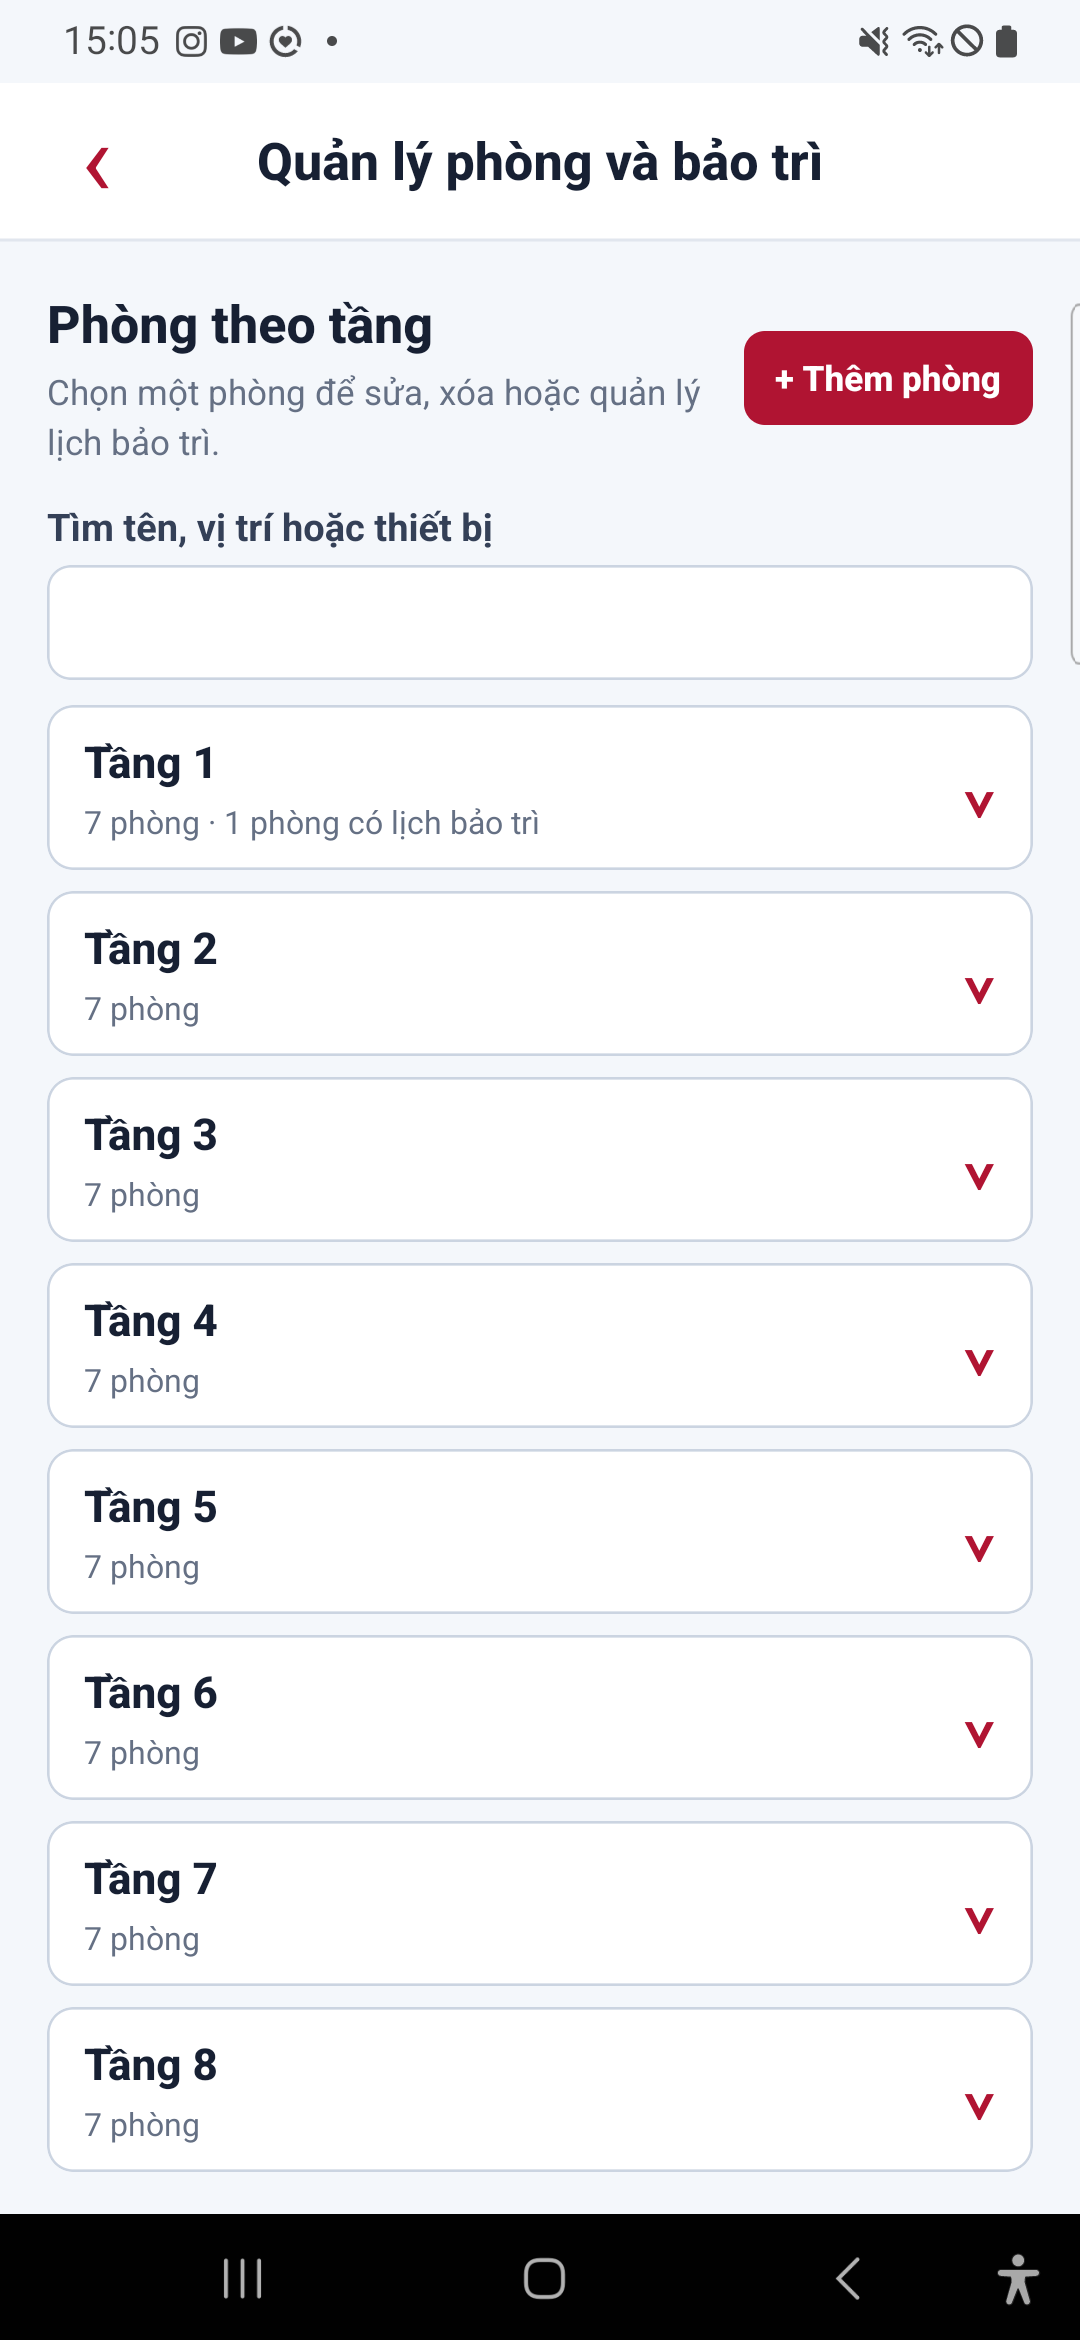
\includegraphics[height=8cm]{Hinhve/quan_ly_phong_theo_tang_hien_tai.png}\hspace{1.2cm}
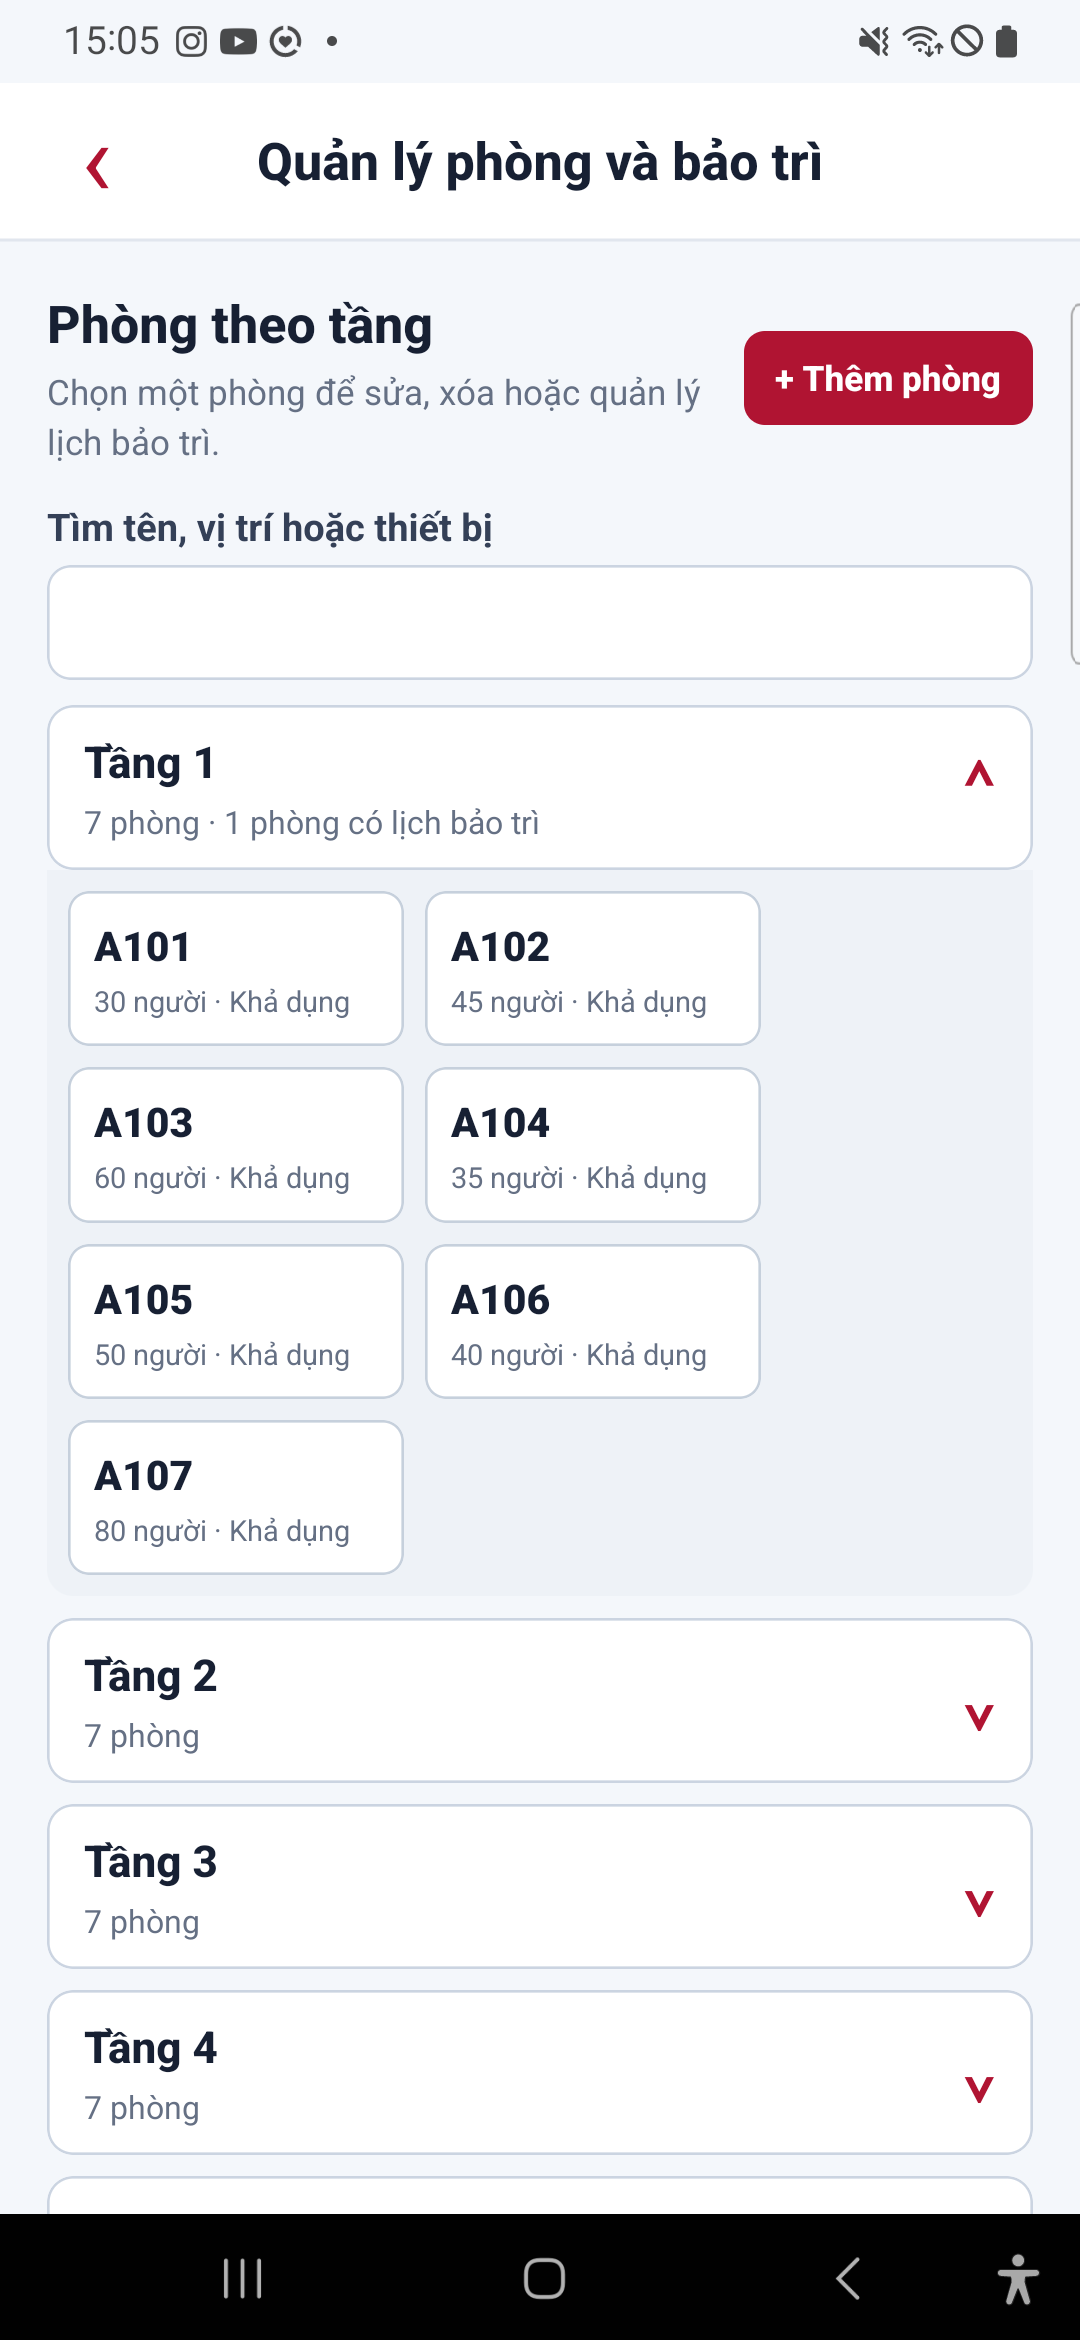
\includegraphics[height=8cm]{Hinhve/phong_tang_mot_hien_tai.png}
\caption{Danh sách tầng và phòng khi mở tầng (trái sang phải)}\label{fig:ui-room-maintenance}
\end{figure}
\subsection{Cấu hình quy tắc đặt phòng}
Hình~\ref{fig:ui-configuration} thể hiện các tham số đặt phòng và công tắc quản trị trên ứng dụng Android. Phần trên gồm cửa sổ đặt trước, hạn mức, hạn hủy/đổi, đệm PIN và ân hạn check-in; phần dưới gồm thông báo hoạt động, tự duyệt phòng thường và nút lưu. Các giá trị được lưu tập trung để dịch vụ nghiệp vụ áp dụng nhất quán. Cấu hình minh họa có min bằng 0, cho phép đặt cùng ngày; giá trị mặc định là 1 ngày. Khi bật tự duyệt, phòng thường được duyệt ngay sau kiểm tra hợp lệ, còn phòng đặc biệt vẫn chờ admin. Kết quả nghiệp vụ được trình bày tại TC07 và TC24.

Form lọc ký tự không phải số; repository vẫn kiểm số nguyên không âm, min không vượt max, hạn mức ít nhất một và quyền admin. Kiểm thử cấu hình xác nhận việc từ chối giá trị vi phạm và thao tác không đủ quyền (TC16).
\begin{figure}[H]\centering
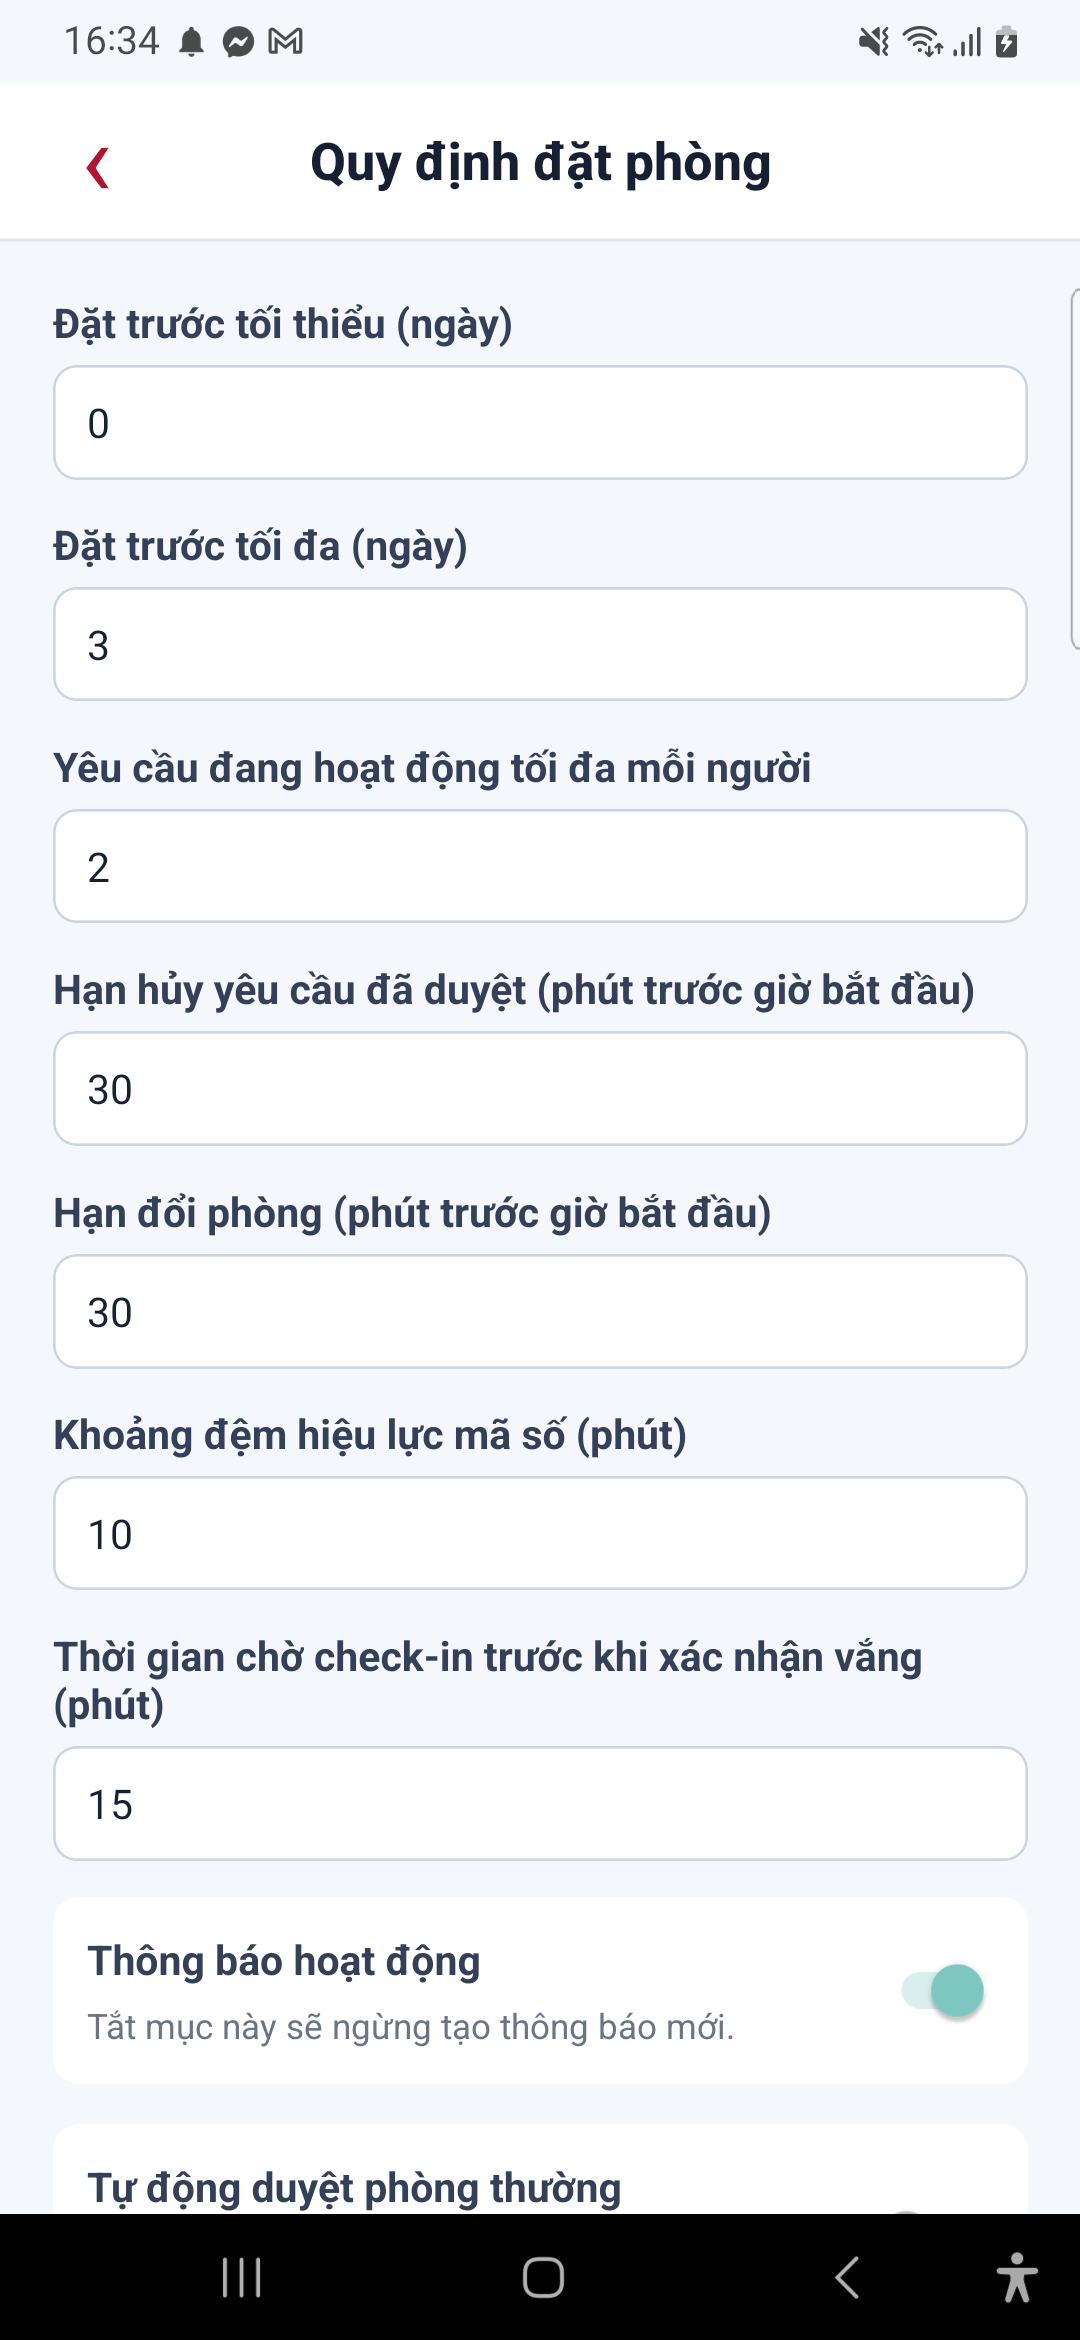
\includegraphics[height=9cm]{Hinhve/cau_hinh_hien_tai.png}\hspace{1cm}
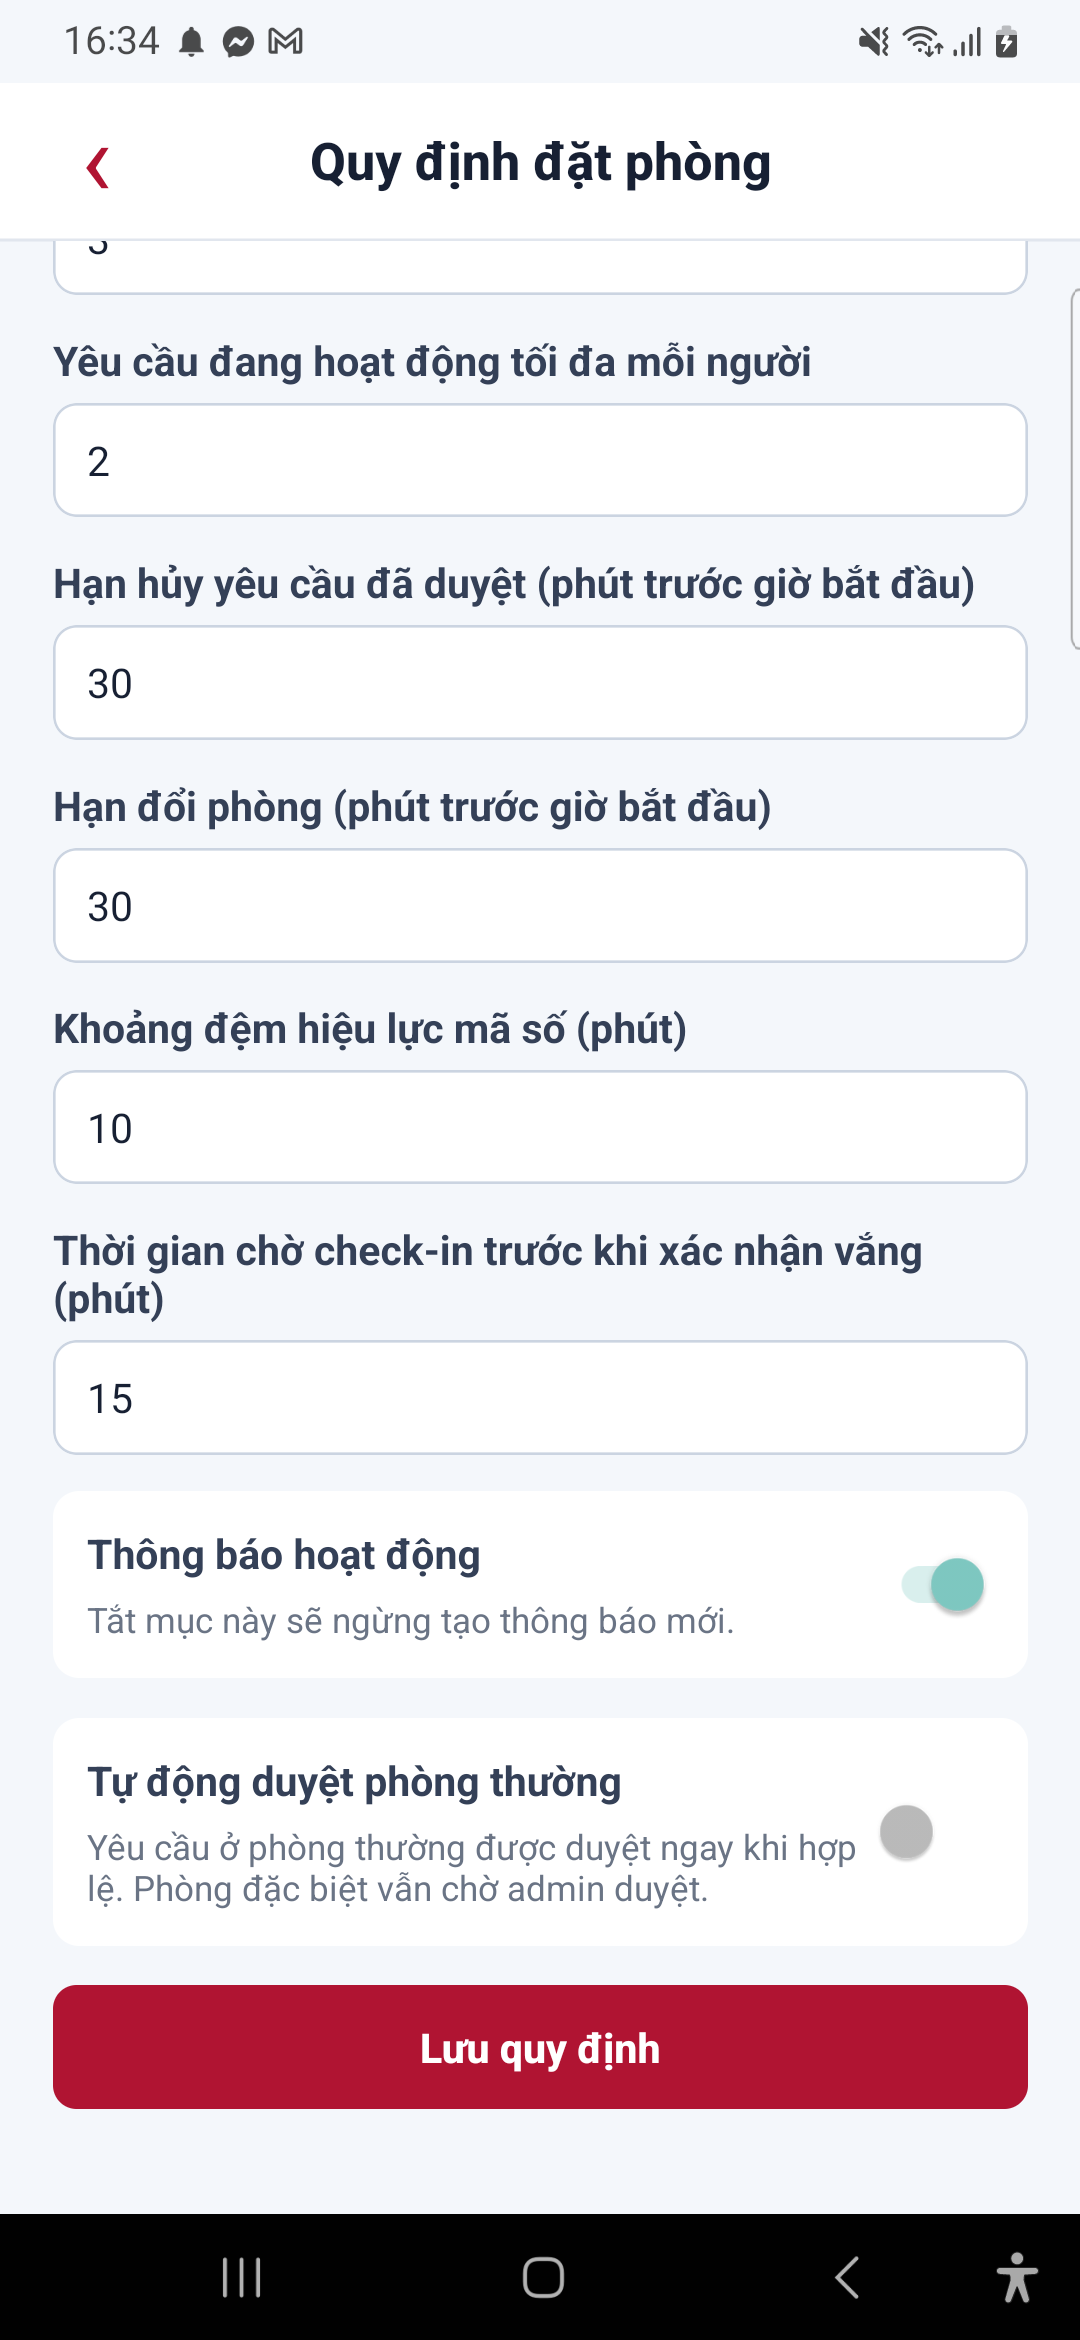
\includegraphics[height=9cm]{Hinhve/cau_hinh_tu_duyet_hien_tai.png}
\caption{Tham số đặt phòng (trái), công tắc thông báo và tự duyệt (phải)}\label{fig:ui-configuration}
\end{figure}
\FloatBarrier

\section{Cấu hình, cài đặt và tái lập bản chạy}
Hình~\ref{fig:deployment} ở Chương~\ref{chap:design} đặt rõ các nơi chạy: APK trên điện thoại, backend/H2 trên máy chủ và kết nối MQTT OneIoT tới khóa. Bảng~\ref{tab:runtime-modes} phân biệt điều kiện sử dụng tương ứng.
{\tabletext\renewcommand{\arraystretch}{1.04}\begin{longtable}{>{\raggedright\arraybackslash}p{\dimexpr0.16\textwidth-2\tabcolsep\relax}>{\raggedright\arraybackslash}p{\dimexpr0.32\textwidth-2\tabcolsep\relax}>{\raggedright\arraybackslash}p{\dimexpr0.52\textwidth-2\tabcolsep\relax}}
\caption{Chế độ chạy, phụ thuộc và phạm vi dữ liệu}\label{tab:runtime-modes}\\
\toprule \textbf{Nhánh} & \textbf{Điều kiện} & \textbf{Hành vi / giới hạn}\\\midrule
\endfirsthead
\multicolumn{3}{l}{\small Chế độ chạy, phụ thuộc và phạm vi dữ liệu (tiếp)}\\
\toprule \textbf{Nhánh} & \textbf{Điều kiện} & \textbf{Hành vi / giới hạn}\\\midrule
\endhead
\bottomrule\endlastfoot
Local & Cờ REST tắt; APK đã có bundle & Đăng nhập và nghiệp vụ dùng Async Storage riêng trên một máy; không cần booking-server. Không tự tải dữ liệu này lên server khi đổi cờ.\\\addlinespace[1.5pt]
REST & Cờ true; backend/URL có thể truy cập từ điện thoại & Repository gọi API, token theo phiên, dữ liệu ở backend. Bản source đang bật nhánh này; URL tunnel trong source là địa chỉ thử nghiệm.\\\addlinespace[1.5pt]
OneIoT & Internet, token Tools trong phiên và khóa gắn với phòng phù hợp & Kết nối MQTT trực tiếp qua native Android, độc lập với cờ REST. PIN được tạo/lưu trước khi gửi; app quản lý metadata gửi lệnh và sự kiện khóa.\\\addlinespace[1.5pt]
\end{longtable}}

\subsection{Cấu hình và dữ liệu khởi tạo}
Cấu hình tại \coderef{code/booking_classroom/src/core/config/runtimeFlags.ts} dùng \code{ENABLE_REMOTE_SYNC=false} cho local, giá trị true cho REST trước khi build; mã nguồn hiện bật REST. Thay đổi cờ hoặc URL được đưa vào JavaScript bundle khi đóng gói lại APK. Local khởi tạo admin/1 và user/2; dữ liệu mẫu chỉ được bổ sung khi kho chưa có, nên cài đè giữ cấu hình và dữ liệu đã lưu.

\subsection{Cài đặt và đóng gói Android}
Tại \code{code/booking_classroom/}, \cmd{npm ci} cài phụ thuộc theo lockfile. Trên Windows, \cmd{npm run build:android:release} tạo bundle, xử lý đường dẫn Unicode qua ổ tạm và gọi Gradle. Trên macOS/Linux, JavaScript được bundle trước khi chạy \cmd{sh ./gradlew assembleRelease} trong thư mục android; cấu hình Release hiện bỏ bước bundle tự động. Quy trình lệnh đầy đủ nằm tại mục~\ref{sec:technical-reproduction} và README gốc repository.

APK đầu ra là \code{android/app/build/outputs/apk/release/app-release.apk}. Sau khi điện thoại cho phép gỡ lỗi USB, cài và mở ứng dụng bằng:
\begin{Verbatim}[fontsize=\small,frame=single,breaklines=true]
adb devices -l
adb install -r android/app/build/outputs/apk/release/app-release.apk
adb shell am start -n com.bookingclassroom/.MainActivity
\end{Verbatim}

Cài đè giữ dữ liệu khi chữ ký tương thích. Bản Release đã đóng gói JavaScript chạy độc lập Metro; chế độ REST cần kết nối backend, còn OneIoT cần mạng và phiên khóa hợp lệ.

\subsection{Backend và kết nối phát triển}
Tại \code{code/booking-server/}, \cmd{mvn spring-boot:run} khởi động dịch vụ cổng 8080 với H2 file. Kết nối qua USB dùng API base URL \code{http://127.0.0.1:8080} và \cmd{adb reverse tcp:8080 tcp:8080}; kết nối Wi-Fi dùng địa chỉ LAN của máy chủ. URL tunnel là địa chỉ tạm thời, phụ thuộc phiên dịch vụ đang chạy.

Bản Debug dùng \cmd{npm start} cho Metro và \cmd{npm run android}; \cmd{adb reverse tcp:8081 tcp:8081} chuyển tiếp cổng Metro qua USB. Cổng 8081 phục vụ JavaScript phát triển, cổng 8080 phục vụ REST. Cơ sở dữ liệu H2 từ xa là lựa chọn bổ sung qua biến BOOKING\_DB; bản local không phụ thuộc cấu hình này.
